\documentclass[pdf]{beamer}
\usepackage[utf8]{vietnam}
\usepackage{amsmath}
\usepackage{amssymb}
\usepackage[utf8]{inputenc}
\usepackage{algorithm,algorithmic}
\usepackage{subfig}
\usepackage{color}
\usepackage{colortbl}
\mode<presentation>{\usetheme{Madrid}}
%\usecolortheme{whale}

%% preamble
\title{Phương pháp học hiệu quả cho mô hình Biterm Topic Model}
%\subtitle{Mô hình Biterm}
\author{Nguyễn Bá Cương}
%\author{Nguyễn Bá Cương\\ Ths Ngô Văn Linh}
\institute[]
{
	Viện Công nghệ thông tin và Truyền thông\\
	Đại học Bách khoa Hà Nội\\ 
		\quad \\
	{\footnotesize Giáo viên hướng dẫn: Ths. Ngô Văn Linh}\\

}

\date[VLC 2017] % (optional)
{Hà Nội 6, 2017}
\begin{document}

%% title frame
\begin{frame}
\titlepage
\end{frame}

\begin{frame}{Nội dung}
\tableofcontents
\end{frame}

\AtBeginSection[]
{
\begin{frame}{Nội dung}
\tableofcontents[currentsection]
\end{frame}
}

%%%%%%%%%%%%%%%%%%%%%%%%%%%%%%%%%%%%%%%%%%%
\section{Short texts và mô hình chủ đề}
\subsection{Short texts}
\begin{frame}{Gới thiệu về short texts}
	Những văn bản ngắn rất là phổ biến trên các trang web 
	\begin{figure}
		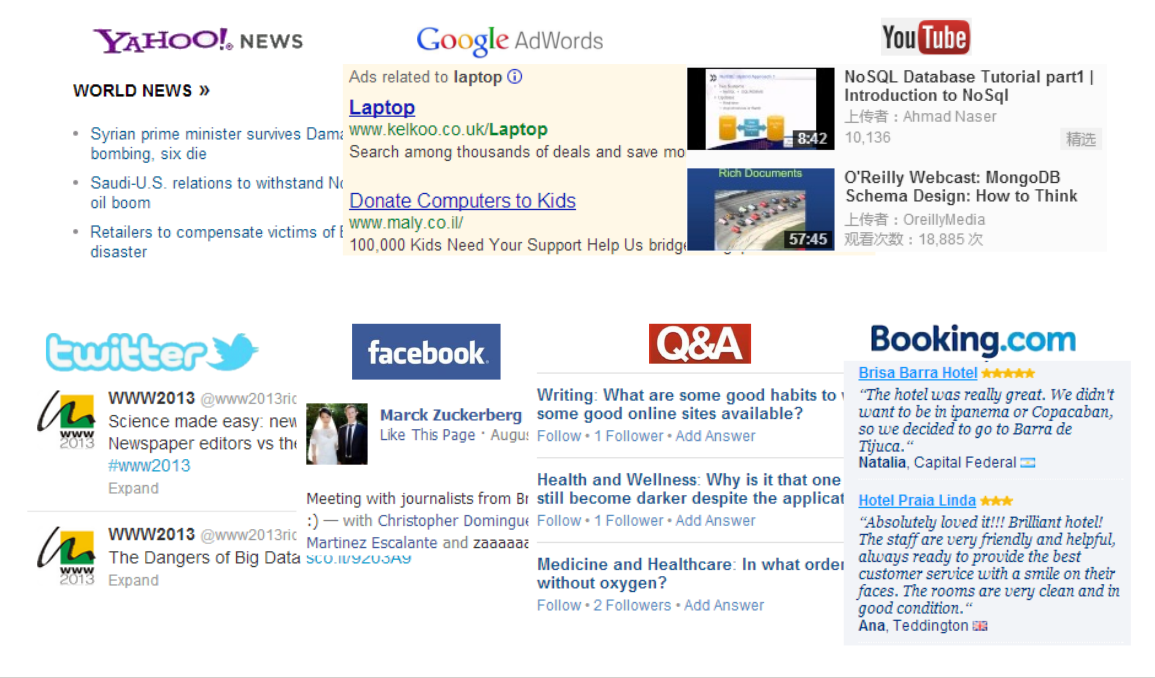
\includegraphics[width=1\textwidth]{01.png}
	\end{figure}
\end{frame}
%
%\begin{frame}{Ứng dụng của short texts}
%Hiểu được chủ đề của các văn bản ngắn rất là quan trong trong nhiều lĩnh vực
%	\begin{itemize}
%		\item Mô tả đặc điểm nội dung (content characterizing)
%		\item Gợi ý nội dung (content recommendation)
%		\item Sở thích người dùng (user interest profiling)
%		\item Phát hiện các chủ đề nổi lên (emerging topic detecting)
%		\item Phân tích ngữ nghĩa (semantic analysic)
%		\item ...
%	\end{itemize}
%\end{frame}

%\begin{frame}{Những vần đề của short texts}
%	Những khó khăn và thách thức
%	\begin{itemize}
%		\item Không đủ ngữ cảnh để xác định ý nghĩa của câu
%		\item Các đặc điểm short texts
%		\begin{itemize}
%			\item Độ dài văn bản rất ngắn
%			\item Số lượng dữ liệu của văn bản ngắn là rất lớn và tăng nhanh
%			\item Các chủ để nó phản ánh đến các xu hướng xã hội
%		\end{itemize}
%		\item Việc giới hạn độ dài của văn bản trong short texts làm cho chúng rất khó để phân tích với các mô hình xác suất truyền thống
%	\end{itemize}
%
%\end{frame}

\subsection{Các mô hình chủ đề}
\begin{frame}{Mô hình chủ đề}
\begin{figure}
	\subfloat[Mô hình chủ đề]{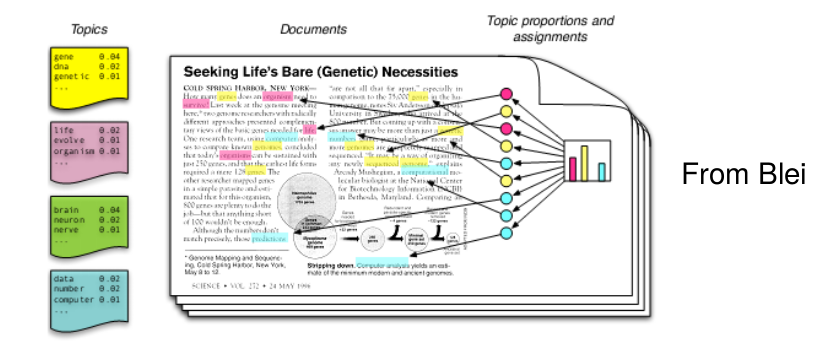
\includegraphics[width=0.7\textwidth]{02.png}}
\end{figure}
Mô hình sinh của các văn bản với chủ đề ẩn
\begin{itemize}
	\item Một chủ đề $\sim$ một phân phối xác suất trong tập từ vựng
	\item Một văn bản $\sim$ một tập trộn của các chủ đề ẩn
	\item Một từ $\sim$ một điểm trong một chủ đề
\end{itemize}	
\end{frame}

\begin{frame}{Mô hình chủ đề truyền thống cho short texts}
Vấn đề: 
	\begin{itemize}
		\item Không đủ ngữ cảnh để xác định ý nghĩa của câu
		\item Các đặc điểm short texts
		\begin{itemize}
			\item Độ dài văn bản rất ngắn
			\item Số lượng dữ liệu của văn bản ngắn là rất lớn và tăng nhanh
			\item Các chủ để nó phản ánh đến các xu hướng xã hội
		\end{itemize}
	\end{itemize}		

	Một số giải pháp:
	\begin{itemize}
		\item Khái thác kiến thức từ bên ngoài để làm giàu sự biểu diễn cho short texts\\
		=> Việc tìm kiếm dữ liệu từ bên ngoài mất nhiều chi phí.
		\item Kết hợp một số văn bản ngắn thành một văn bản dài dựa trên một số thông tin. Như tập hợp các bài đăng trên Twitter bời cùng một người dùng, hay cùng hashtags.
		\\=> Việc làm này là không mang tính tổng quát
	\end{itemize}

\end{frame}
%\begin{frame}{Mô hình Mixture of Unigrams}
%\begin{columns}[T] % align columns
%	\begin{column}{.50\textwidth}
%		\begin{itemize}
%			\item Giả định rằng tất cả các từ thuộc một văn bản đều thuộc cùng một chủ đề\\
%			=> Vấn đề: Mặc dù là short text nhưng mỗi văn bản vẫn có thể có nhiều hơn 1 chủ đề
%			%			\item trong khi chủ đề $z$ được lấy mẫu từ một tỉ lệ chủ đề toàn cục $\theta$
%		\end{itemize}
%	\end{column} %
%	\hfill%	
%	\begin{column}{.50\textwidth}
%		\begin{figure}
%			\subfloat[Mô hình Mixture of unigrams]{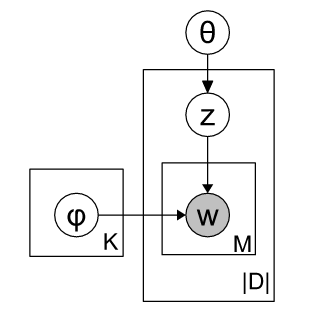
\includegraphics[width=0.85\textwidth]{Mix.png}}
%		\end{figure}				
%	\end{column} %
%\end{columns}
%$\hspace{5cm}$
%\end{frame}
\begin{frame}{Mô hình Biterm Topic Model (BTM)}
Ý tưởng chính
\begin{columns}[T] % align columns
	\begin{column}{.55\textwidth}
		\begin{itemize}
		\item Chủ đề là tập các từ tương đồng. Các từ cùng xuất hiện trong cùng một văn bản
		\\=> Tại sao không mô hình trực tiếp các từ đồng xuất hiện để học các chủ đề.
		\item Mô hình chủ đề chịu nhiều vấn đề từ văn bản ngắn 
		\\=> Tại sao không sử dụng toàn toàn bộ dữ liệu.
		\end{itemize}
	\end{column} %
	\hfill%	
	\begin{column}{.43\textwidth}
		\begin{figure}
			\subfloat[Mô hình BTM]{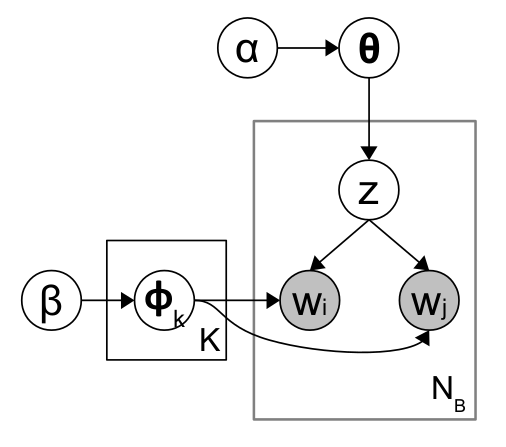
\includegraphics[width=1\textwidth]{BTM.png}}
		\end{figure}				
	\end{column} %
\end{columns}

\end{frame}
%\begin{frame}{Mô hình Biterm Topic Model (BTM)}
%\begin{itemize}
%	\item Biterm là một cặp từ không theo thứ tự cùng xuất hiện trong một văn bản \\
%	\begin{center}
%	\centering Ví dụ như một văn bản gồn có 3 từ $w_1, w_2, w_3$ thì biterm là \\
%	\centering $(w_1, w_2, w_3) \overrightarrow{} \{(w_1, w_2), (w_2, w_3), (w_1, w_3)\} $
%	\end{center}
%	\item Dữ liệu học tập hợp tất cả các biterm được sinh từ mỗi văn bản
%\end{itemize}
%\end{frame}

%
%\begin{frame}{Mô hình BTM}
%\begin{figure}
%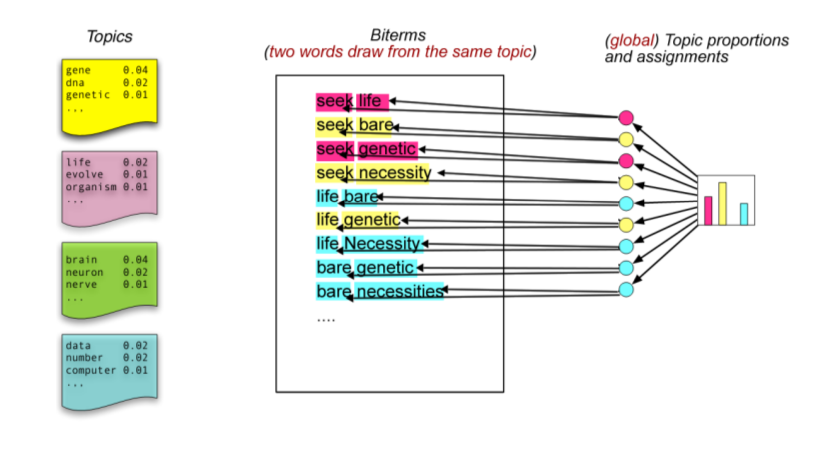
\includegraphics[width=0.7\textwidth]{06.png}
%\end{figure}				
%Mô hình sinh của biterms với chủ đề ẩn
%\begin{itemize}
%\item Chủ đề $\sim$ phân phối qua các từ 
%\item Tập dữ liệu $\sim$ tập trộn các chủ đề
%\item Một biterm $\sim$ hai từ xác định biểu diển cùng trong một chủ đề
%\end{itemize}
%\end{frame}

%%%%%%%%%%%%%%%%%%%%%%%%%%%%%%%%%%%%%%%%%%%
\section{Phương pháp học mới cho mô hình BTM}

\subsection{Phương pháp Gibbs-sampling}
\begin{frame}{Phương pháp Gibbs Sampling}
\begin{itemize}
	\item Ý tưởng: Sinh ra một mẫu phân bố hậu nghiệm bằng cách duyệt qua các giá trị từ tập dữ liêu ban đầu.
%	\item Ví dụ:\\
%	Cho các biến ngẫu nhiên $X_1, X_2, X_3$\\
%	Khởi tạo: $x_1^{(0)}, x_2^{(0)}, x_3^{(0)}$ \\
%	Tại bước lặp thứ $i$
%	\begin{align*}
%	x_1^{(i)} = p(X_1 = x_1| X_2 = x_2^{(i-1)},  X_3 = x_3^{(i-1)})\\
%	x_2^{(i)} = p(X_2 = x_2| X_1 = x_1^{(i)},  X_3 = x_3^{(i-1)}) \\
%	x_3^{(i)} = p(X_3 = x_3| X_1 = x_1^{(i)},  X_2 = x_2^{(i)}) 
%	\end{align*}
%	Qúa trình này sẽ dừng đến khi hội tụ
	\item Vấn đề của phương pháp Gibbs-sampling
		\begin{itemize}
			\item Không xác định được thời gian hội tụ
			\item Dữ liệu biterm sinh ra quá lớn\\
			=> Gibbs-sampling cho thời gian chạy rất lâu.
		\end{itemize} 
\end{itemize}
\end{frame}
%
%\begin{frame}{Áp dụng cho mô hình BTM}
%Lấy mẫu chủ đề cho từng biterm trong mini-batch $t$
%\begin{align}
%P(z_i = k|z_{-i}^{(t)}, B^{(t)}, \alpha^{(t)}, \{\beta_k^{(t)}\}_{k=1}^K) \propto  \nonumber \\
%(n_{-i, k} ^{(t)}, \alpha_k^{(t)})\dfrac{(n_{-i, w_i|k}^{(t)} + \beta_{k, w_i}^{(t)})(n_{-i, w_j|k}^{(t)} + \beta_{k, w_j}^{(t)})}{[\sum_{w=1}^W(n_{-i, w|k}^{(t)} + \beta_{k, w}^{(t)})]^2} 
%\end{align}
%Cập nhật lại các tham số
%\begin{align}
%\alpha_k^{(t+1)} = \alpha_k^{(t)} + \lambda n_k^{(t)} \\
%\beta_{k, w}^{(t+1)} = \beta_{k, w} ^{(t)} + \lambda n_{w|k}^{(t)} \\
%\phi_{k,w}^{(t)} = \dfrac{n_{w|k}^{(t)} + \beta^{(t)}}{n_{.|k}^{(t)} + W\beta^{(t)}} \\
%\theta_k^{(t)} = \dfrac{n_k^{(t)} + \alpha^{(t)}}{N_\beta^{(t)} + K\alpha^{(t)}}
%\end{align}
%\end{frame}

%\begin{frame}
%\begin{algorithm}[H]
%\textbf{Input: }  $K, \alpha , \beta, $ biterm sets $B^{(1)}, ..., B^{(T)}$  \\
%\textbf{Output:} $\{\phi^{(t)}, \theta^{(t)} \}_{t=1}^T$
%\begin{algorithmic}[1]
%\STATE {Set $\alpha^{(1)} = {(\alpha, ..., \alpha)}$ and $\{\beta_k^{(1)} = {(\beta, ..., \beta)}\}_{k = 1}^K$}
%\FOR{$t =1$ to $T$ do}
%\STATE {Randomly initialize the topic asignments for all the biterms}
%\FOR{$iter=1$ to $N_{iter}$ do}
%\FOR{\textbf{each} biterm $b_i = {(w_{i, 1}, w_{i,2})} \ni B^{(t)} $}
%\STATE {Drawn topic k from Eq.(2)}
%\STATE {Update $n_k^{(t)}, n_{w_{i,1}|k}^{(t)}$ and $n_{w_{i,2}|k}^{(t)}$}
%\ENDFOR
%\STATE {$\alpha^{(t+1)}$ and $\{\beta_k^{(t+1)}\}_{k=1}^{K}$ by Eq.(3)and Eq.(4)}
%\ENDFOR
%\STATE {Compute $\phi^{(t)}$ by Eq.(5) and $\theta^{(t)}$ by Eq.(6)}
%\ENDFOR
%\end{algorithmic}
%\caption{Thuật toán Gibbs sampling dạng online cho mô hình BTM }
%\end{algorithm}
%\end{frame}

%\begin{frame}{Phương pháp học mới}
%	\begin{itemize}
%		\item Vấn đề của phương pháp Gibbs-sampling
%			\begin{itemize}
%				\item Không xác định được thời gian hội tụ
%				\item Dữ liệu biterm sinh ra quá lớn\\
%				=> Gibbs-sampling cho thời gian chạy rất lâu.
%			\end{itemize} 
%		\item Giải pháp
%			\begin{itemize}
%			\item Phương pháp suy diễn biến phân (VB) \\
%			\item Phương pháp học ngẫu nhiên (RVB)
%			\end{itemize} 
%	\end{itemize}
%\end{frame}
\subsection{Phương pháp suy diễn biến phân}
\begin{frame}{Phương pháp suy diễn biến phân (VB)}
\begin{itemize}
	\item Thay vì tối ưu hóa trực tiếp hàm mục tiêu, ta xây dựng một
	cận dưới cho hàm mục tiêu và tối ưu hóa trên cận dưới đó.
%	\item Tuy nhiên nếu lower-bound đủ chặt, giá trị tham số mới tìm được sẽ
%	đảm bảo tốt hơn giá trị cũ
	\item Thuật toán thực hiện hai bước như sau
	\begin{itemize}
		\item Bước E ta tính giá trị
		\begin{align*}
		t_{n,k} &=  \frac{\phi_{k,w_{n,1}} \phi_{k,w_{n,2}} \theta_k}
		{\sum_k \phi_{k,w_{n,1}} \phi_{k,w_{n,2}} \theta_k}
		\end{align*}
		
		\item Bước M ta cập nhật giá trị
		\begin{align*}
		\theta_k &= \frac{\sum_n t_{n,k} + \alpha}{\sum_{k'} \big( \sum_n t_{n,k'} + \alpha \big)} \\
		\phi_{k,w} &= \frac{\sum_{n} t_{n,k} \ c(b_{n},w) + \beta}{W \beta + \sum_{n} 2t_{n,k}}
		\end{align*}
	\end{itemize}				
\end{itemize}

%\begin{figure}
%	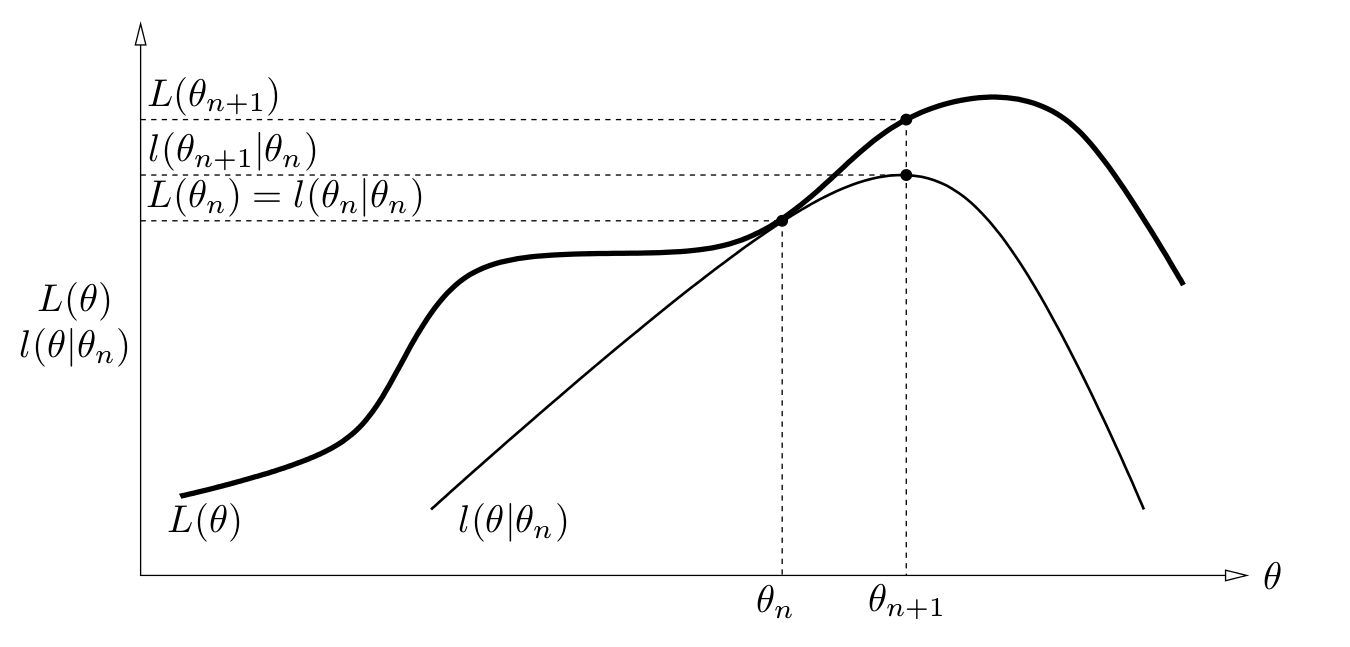
\includegraphics[scale=0.2]{lower.png}
%\end{figure}
\end{frame}

%\begin{frame}{Phương pháp suy diễn biến phân}
%%Hàm lower-bound:
%%\begin{align*}
%%\mathcal{L}(Q, \theta) = & \sum_i^N \sum_{z_{i}} P(z_{i}|x_{i},\theta^{old}) \log P(x_{i}z_{i}|\theta) \\
%%& - \sum_i^N \sum_{z_{i}} P(z_{i}|x_{i},\theta^{old}) \log P(z_{i}|x_{i},\theta^{old}) + \log P(\theta)
%%\end{align*}
%Thuật toán thực hiện hai bước như sau
%\begin{itemize}
%	\item Bước E ta tính giá trị
%	\begin{align*}
%	t_{n,k} &=  \frac{\phi_{k,w_{n,1}} \phi_{k,w_{n,2}} \theta_k}
%	{\sum_k \phi_{k,w_{n,1}} \phi_{k,w_{n,2}} \theta_k}
%	\end{align*}
%
%	\item Bước M ta cập nhật giá trị
%	\begin{align*}
%	\theta_k &= \frac{\sum_n t_{n,k} + \alpha}{\sum_{k'} \big( \sum_n t_{n,k'} + \alpha \big)} \\
%	\phi_{k,w} &= \frac{\sum_{n} t_{n,k} \ c(b_{n},w) + \beta}{W \beta + \sum_{n} 2t_{n,k}}
%	\end{align*}
%\end{itemize}
%\end{frame}
\begin{frame}
\begin{algorithm}[H]
%	Define $ \gamma_i = (i+2)^{-p}$ \\
	\textbf{Input: } Số lượng chủ đề $K, \alpha, \beta, \{\gamma_i\}_{i = 1}^T$, tập dữ liệu $B^{(1)}, ..., B^{(T)}$  \\
	\textbf{Output: } $\phi, \theta$ 
	\begin{algorithmic}[1]
		\STATE Khởi tạo ngẫu nhiên $\phi, \theta,  S_{\theta_k}^0 = 0, S_{\phi_{k, w}}^0 = 0, i = 0$
		\FOR{$i=1$ to $\infty$}
		\FOR{\textbf{each} biterm $b_j = (w_{i, 1}, w_{i,2}) \ni B^{(i)} $}
		\STATE $ t_{j, k} \propto {\phi_{k,w_{j,1}} \phi_{k,w_{j,2}} \theta_k}$
		\ENDFOR
		\STATE  $S_{\phi_{k, w}}^i = \sum_{j}{t_{i, k}c(b_j, w)}$ ; \space  $S_{\theta_k}^i = \sum_{j}{t_{j, k}} $
%		#update
		\STATE$S_{\phi_{k, w}}^i = (1 - \gamma_i) S_{\phi_{k, w}}^{(i-1)} + \gamma_i S_{\phi_{k, w}}^i$; \space $S_{\theta_k}^i = (1 - \gamma_i)S_{\theta_k}^{(i-1)} + \gamma_i S_{\theta_k}^i$\\ \#Cập nhật tham số mô hình
		\STATE $\theta_k \propto S_{\theta_k}^i + \alpha$ ; \space $\phi_{k, w} \propto S_{\phi_{k, w}}^i + \beta $
		\ENDFOR
	\end{algorithmic}
	\caption{Thuật toán Online VB cho mô hình BTM }
\end{algorithm}
\end{frame}
\subsection{Phương pháp học ngẫu nhiên}
\begin{frame}{Phương pháp học ngẫu nhiên}
%	Học một cách ngẫu nhiên một lượng các biterm trên tập dữ liệu ban đầu (các biterm):
%	Với mỗi minibatch chọn ngẫu nhiên một lượng biterm bằng cách sử dụng phân phối nhị thức với một xác suất p.
	\begin{itemize}
		\item Trong quá trình học, ở mỗi minibatch, chúng ta bỏ đi một phần dữ liệu của minibatch đó.
		\begin{itemize}
			\item Dữ liệu bỏ đi là một cách ngẫu nhiên. Bỏ đi từng biterm trong tập dữ liệu với xác suất là p.
			\item Ở mỗi vòng lặp, dữ liệu bỏ đi không được sử dụng.
		\end{itemize}
		\item Ý tưởng này áp dụng rộng cho nhiều phương pháp học khác.
			\begin{itemize}
			\item Áp dụng cho phương pháp VB => RVB
			\item Áp dụng cho phương pháp Gibbs-sampling => R-Gibbs-sampling
		\end{itemize}
	\end{itemize}
\end{frame}
\begin{frame}
\begin{algorithm}[H]
%	Define $ \gamma_i = (i+2)^{-p}$ \\
	\textbf{Input: } Số lượng chủ đề $K, \alpha, \beta, \{\gamma_i\}_{i = 1}^T$, tập dữ liệu $B^{(1)}, ..., B^{(T)}, p$  \\
	\textbf{Output: } $\phi, \theta$ 
	\begin{algorithmic}[1]
		\STATE Khởi tạo ngẫu nhiên $\phi, \theta,  S_{\theta_k}^0 = 0, S_{\phi_{k, w}}^0 = 0, i = 0$
		\FOR{$i=1$ to $\infty$}
		\STATE Chọn một lượng các biterm trong mỗi mini-batch $B^{(i)}$. \\
		Mỗi biterm trong minibatch thì khả năng bỏ đi là một giá trị xác suất $p$. Tập dữ liệu sau khi bỏ đi là $C$
		\FOR{\textbf{each} biterm $b_j = (w_{i, 1}, w_{i,2}) \ni C $}
		\STATE $ t_{j, k} \propto {\phi_{k,w_{j,1}} \phi_{k,w_{j,2}} \theta_k}$
		\ENDFOR
		\STATE  $S_{\phi_{k, w}}^i = \sum_{j}{t_{i, k}c(b_j, w)}$ ; \space  $S_{\theta_k}^i = \sum_{j}{t_{j, k}} $
		%		#update
		\STATE$S_{\phi_{k, w}}^i = (1 - \gamma_i) S_{\phi_{k, w}}^{(i-1)} + \gamma_i S_{\phi_{k, w}}^i$; \space $S_{\theta_k}^i = (1 - \gamma_i)S_{\theta_k}^{(i-1)} + \gamma_i S_{\theta_k}^i$
		\STATE $\theta_k \propto S_{\theta_k}^i + \alpha$ ; \space $\phi_{k, w} \propto S_{\phi_{k, w}}^i + \beta $
		\ENDFOR
	\end{algorithmic}
	\caption{Thuật toán Online RVB cho mô hình BTM}
\end{algorithm}
\end{frame}
%
%\begin{frame}
%\begin{algorithm}[H]
%	\textbf{Input: }  $K, \alpha , \beta, $ biterm sets $B^{(1)}, ..., B^{(T)}$  \\
%	\textbf{Output:} $\{\phi^{(t)}, \theta^{(t)} \}_{t=1}^T$
%	\begin{algorithmic}[1]
%		\STATE {Set $\alpha^{(1)} = {(\alpha, ..., \alpha)}$ and $\{\beta_k^{(1)} = {(\beta, ..., \beta)}\}_{k = 1}^K$}
%		\FOR{$t =1$ to $T$ do}
%		\STATE {Randomly initialize the topic asignments for all the biterms}
%		\FOR{$iter=1$ to $N_{iter}$ do}
%		\STATE {\color{blue}{Generating minibatch $B^{`(t)}$ from $B^{(t)}$}}
%		\FOR{\textbf{each} biterm $b_i = {(w_{i, 1}, w_{i,2})} \ni B^{`(t)} $}
%		\STATE {Drawn topic k from Eq.(1)}
%		\STATE {Update $n_k^{(t)}, n_{w_{i,1}|k}^{(t)}$ and $n_{w_{i,2}|k}^{(t)}$}
%		\ENDFOR
%		\STATE {$\alpha^{(t+1)}$ and $\{\beta_k^{(t+1)}\}_{k=1}^{K}$ by Eq.(2)and Eq.(3)}
%		\ENDFOR
%		\STATE {Compute $\phi^{(t)}$ by Eq.(4) and $\theta^{(t)}$ by Eq.(5)}
%		\ENDFOR
%	\end{algorithmic}
%	\caption{Online BTM Algorithm }
%	\label{alg:seq}
%\end{algorithm}
%\end{frame}


\begin{frame}
\begin{algorithm}[H]
	\textbf{Input: }  $K, \alpha , \beta, $ tập dữ liệu $B^{(1)}, ..., B^{(T)}, p$  \\
	\textbf{Output:} $\{\phi^{(t)}, \theta^{(t)} \}_{t=1}^T$
	\begin{algorithmic}[1]
		\STATE {Khởi tạo $\alpha^{(1)} = {(\alpha, ..., \alpha)}$ và $\{\beta_k^{(1)} = {(\beta, ..., \beta)}\}_{k = 1}^K$}
		\FOR{$t =1$ to $T$}
		\STATE {Khởi tạo ngẫu nhiên các giá trị chủ để cho tất cả các biterm}
		\FOR{$iter=1$ to $N_{iter}$}
		\STATE Chọn một lượng các biterm trong mỗi mini-batch $B^{(t)}$. \\
		Mỗi biterm trong minibatch thì khả năng bỏ đi là một giá trị xác suất $p$. 
		Tập dữ liệu sau khi bỏ đi là $C$
		\FOR{\textbf{each} biterm $b_i = {(w_{i, 1}, w_{i,2})} \ni C $}
		\STATE {Tính giá trị $k$ và cập nhật $n_k^{(t)}, n_{w_{i,1}|k}^{(t)}$ và $n_{w_{i,2}|k}^{(t)}$ theo $k$}
		\ENDFOR
		\STATE {Cập nhật $\alpha^{(t+1)}$  và $\{\beta_k^{(t+1)}\}_{k=1}^{K}$}
		\ENDFOR
		\STATE {Cập nhật $\phi^{(t)}$ và $\theta^{(t)}$ }
		\ENDFOR
	\end{algorithmic}
	\caption{Thuật toán Online R-Gibbs-sampling cho mô hình BTM }
	\label{alg:seq}
\end{algorithm}
\end{frame}

\begin{frame}{Những điểm mạnh của phương pháp học mới}
Phương pháp VB:
	\begin{itemize}
		\item Thời gian học của phương pháp VB nhanh hơn so với phương pháp \textit{Gibbs-sampling} mà tác giả đề xuất.
		\item \textit{VB} cho chất lượng mô hình cao hơn so với phương pháp học bằng \textit{Gibbs-sampling}
	\end{itemize}
Phương pháp học ngẫu nhiên:
	\begin{itemize}
		\item Phương pháp học ngẫu nhiên cho thời gian chạy nhanh hơn so với phương pháp gốc thực hiện.
		\item Phương pháp học ngẫu nhiên cho chất lượng chủ đề xấp xỉ như kết quả mà phương pháp gốc thực hiện
	\end{itemize}
\end{frame}

%%%%%%%%%%%%%%%%%%%%%%%%%%%%%%%%%%%%%%%%%%%
\section{Thử nghiệm - Đánh giá}
\subsection{Dữ liệu thử nghiệm}
\begin{frame}{Bộ dữ liệu thử nghiệm}
\begin{table}
	\begin{tabular}{l | c | c | c }
%		& Corpus size & Average length per doc & V \\
		& Số lương văn bản & Độ dài trung bình & V \\
		\hline \hline
		Twitter & 1,485,068 & 10.14 & 89,474 \\
		Yahoo Questions & 537,770 & 4.73 & 24,420  \\ 
		Nytimes Titles & 1,684,127 & 5.15 & 55,488
	\end{tabular}
	\caption{Bảng mô tả dữ liệu thử nghiệm}
\end{table}
\end{frame}
\begin{frame}{Tiêu chí đánh giá}
	\begin{itemize}
		\item Thử nghiệm so sánh trên 3 phương pháp: 
		\begin{itemize}
			\item Gibbs-sampling
			\item Suy diễn biến phân - VB
			\item Học ngẫu nhiên: Phương pháp RVB và R-Gibbs-sampling
		\end{itemize}
		\item Tiêu chí đánh giá:
		\begin{itemize}
			\item Khả năng phán đoán mô hình: Sử dụng độ đo \textit{log predictive probability}
			\item Chất lượng chủ đề: Sử dụng độ đo NPMI
			\item Thời gian chạy
		\end{itemize}
	\end{itemize}
\end{frame}
\subsection{Kết quả thử nghiệm}

\begin{frame}{Độ đo khả năng phán đoán mô hình}
	
\begin{columns}[T] % align columns
	\begin{column}{.50\textwidth}
		\begin{figure}
			\subfloat[Online Gibbs-sampling và R-Gibbs-sampling]{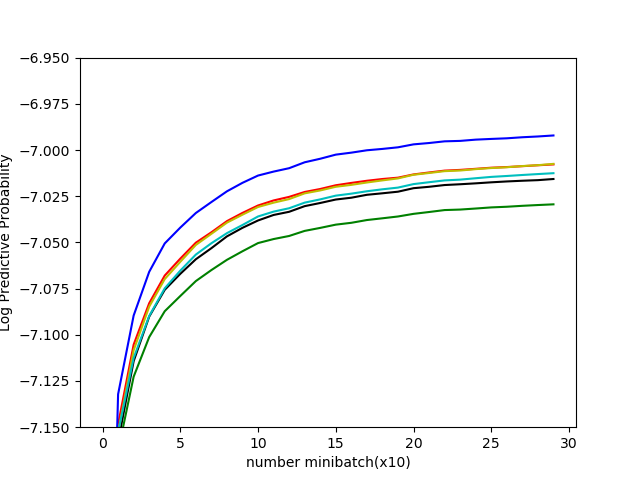
\includegraphics[width=1.1\textwidth]{twitterPer100gibb.png}}
		\end{figure}
	\end{column} %
	\hfill%	
	\begin{column}{.50\textwidth}
		\begin{figure}
			\subfloat[Online VB và RVB]{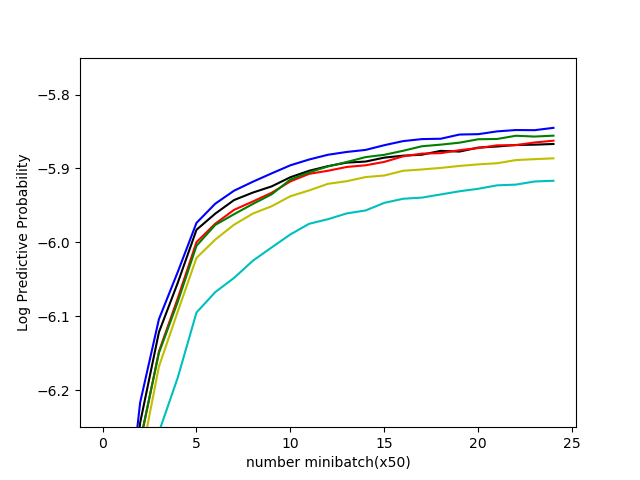
\includegraphics[width=1.1\textwidth]{twitterPer100vb.png}}
		\end{figure}				
	\end{column} %
\end{columns}
%\begin{center}
%	
\includegraphics[width=1\textwidth]{menu.png}	
%\end{center}

  \begin{figure}
	\begin{center}
		\captionsetup{justification=centering}
		
\includegraphics[width=100mm]{menu.png}
		\caption{Kết quả độ đo khả năng phán đoán mô hình cho bộ dữ liệu Twitter}
	\end{center}
\end{figure}

\end{frame}

\begin{frame}{Độ đo chất lượng chủ đề }
\begin{columns}[T] % align columns
\begin{column}{.50\textwidth}
	\begin{figure}
		\subfloat[Online Gibbs-sampling và R-Gibbs-sampling]{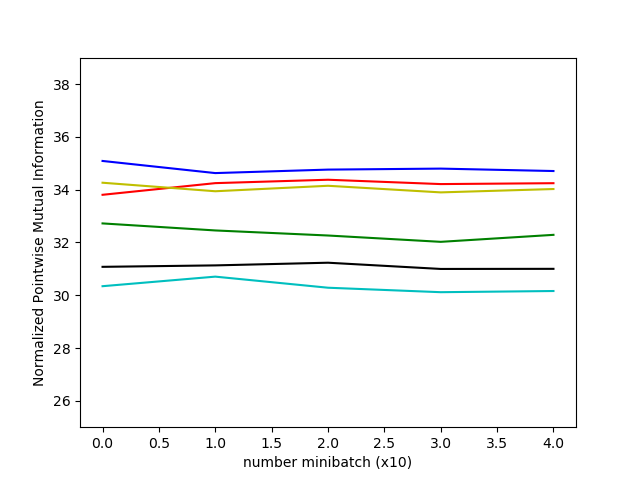
\includegraphics[width=1.1\textwidth]{twitterNPMI100gibb.png}}
	\end{figure}
\end{column} %
\hfill%	
\begin{column}{.50\textwidth}
	\begin{figure}
		\subfloat[Online VB và RVB]{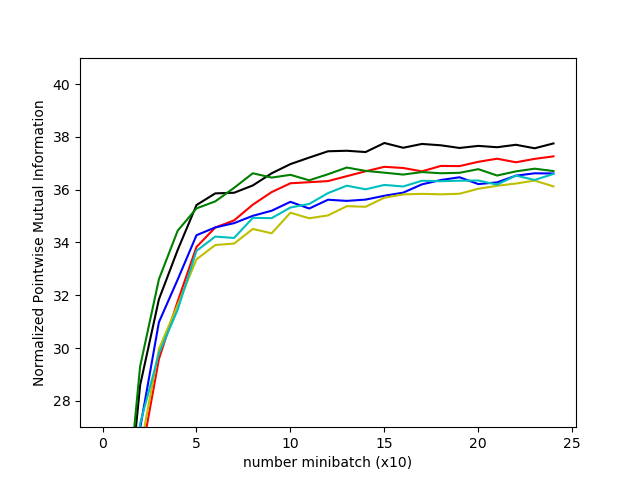
\includegraphics[width=1.1\textwidth]{twitterNPMI100vb.png}}
	\end{figure}				
\end{column} %
\end{columns}

\begin{figure}
	\begin{center}
		\captionsetup{justification=centering}
		
\includegraphics[width=100mm]{menu.png}
		\caption{Kết quả độ đo chất lượng chủ đề cho bộ dữ liệu Twitter}
	\end{center}
\end{figure}
\end{frame}

\begin{frame}{Thời gian huấn luyện}
		\begin{tabular}{l|c |c | c | c | c | c | c }
		& K & origin & p = 0.1 & p = 0.3 & p = 0.5 & p = 0.7 & p = 0.9 \\
		\hline \hline
		Gibbs &50 & 249935& 231575 & 186822 & 80132 & 56739 & 24534 \\ 
		\hline
		VB &50 & 3592& 3463 & 2922 & 2166 &1249 & 375 \\
		\hline \hline
		Gibbs &100 &404573 & 357891 & 288019 & 213525 & 134510&  46840\\ 
		\hline
		VB &100 &3224 & 3050 & 2503 & 1870 &1189 &880\\
		\hline \hline
		Gibbs &150 &460189 & 429685 & 350120 & 297817 & 296984& 114108 \\ 
		\hline
		VB &150 &3866 & 3696 & 3052 & 2429 &1536 &781\\
		\hline \hline
		Gibbs &200 & 539904& 538529 & 456806 & 387955 & 275327 & 171603 \\ 
		\hline
		VB &200 &4925 & 4594 & 3313 & 2622 & 1944&1322\\
	\end{tabular}
\end{frame}

\begin{frame}{Đánh giá}
	\begin{itemize}
		\item Phương pháp Gibbs sampling, cho thời gian chạy rất chậm.
		\item Phương pháp VB cho thời học vượt trội hơn hẳn, và kết quả chất lượng mô hình cao hơn so với phương pháp học Gibbs sampling.
		\item Phương pháp học ngẫu nhiên cho thời gian học nhanh hơn nhiều lần ứng với lượng dữ liệu được bỏ đi.
	\end{itemize}
\end{frame}
%%%%%%%%%%%%%%%%%%%%%%%%%%%%%%%%%%%%%%%%%%%
\section{Kết luận}
	\begin{frame}{Kết luận}
		\begin{itemize}
			\item Phương pháp học VB 
			\begin{itemize}
				\item  Kết quả cho thấy chất lượng chủ đề hay khả năng phán đoán của mô hình tốt hơn hẳn so với  phương pháp Gibbs sampling
				\item  Thời gian học của phương pháp VB vượt trội hơn hẳn so với phương pháp Gibbs-sampling
			\end{itemize}
		\item Phương pháp học ngẫu nhiên
			\begin{itemize}
				\item Chất lượng mô hình xấp xỉ với phương pháp gốc.
				\item Thời gian học nhanh hơn rất nhiều so với phương pháp gốc.
			\end{itemize}
		\end{itemize}
	\end{frame}
%\begin{frame}
%\frametitle{A first slide}

\begin{figure}
	\begin{center}
		
\includegraphics[width=110mm]{thankyou.jpg}
	\end{center}
\end{figure}

%\end{frame}
%
\begin{frame}{Độ đo khả năng phán đoán mô hình}
%	K = 100, sử dụng độ đo perplexity 
	\begin{columns}[T] % align columns
		\begin{column}{.50\textwidth}
		\begin{figure}
			\subfloat[Online Gibbs-sampling và R-Gibbs-sampling]{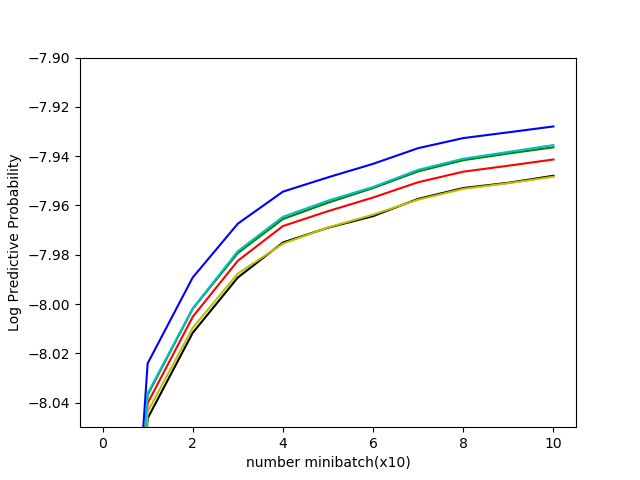
\includegraphics[width=1.1\textwidth]{yahooPer100gibb.png}}
		\end{figure}
		\end{column} %
		\hfill%	
		\begin{column}{.50\textwidth}
			\begin{figure}
				\subfloat[Online VB và RVB]{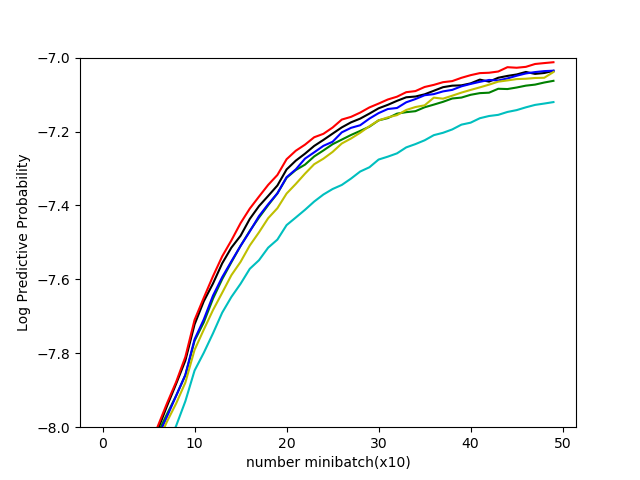
\includegraphics[width=1.1\textwidth]{yahooPer100vb.png}}
			\end{figure}				
		\end{column} %
	\end{columns}
 \begin{figure}
	\begin{center}
		\captionsetup{justification=centering}
		
\includegraphics[width=100mm]{menu.png}
		\caption{Kết quả độ đo khả năng phán đoán mô hình cho bộ dữ liệu Yahoo}
	\end{center}
\end{figure}
\end{frame}

\begin{frame}{Độ đo chất lượng chủ đề }
\begin{columns}[T] % align columns
	\begin{column}{.50\textwidth}
		\begin{figure}
			\subfloat[Online Gibbs-sampling và R-Gibbs-sampling]{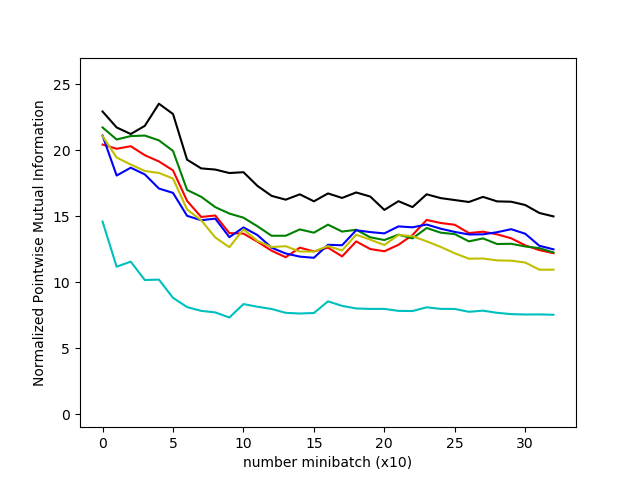
\includegraphics[width=1.1\textwidth]{yahooNPMI100gibb.png}}
		\end{figure}
	\end{column} %
	\hfill%	
	\begin{column}{.50\textwidth}
		\begin{figure}
			\subfloat[Online VB và RVB]{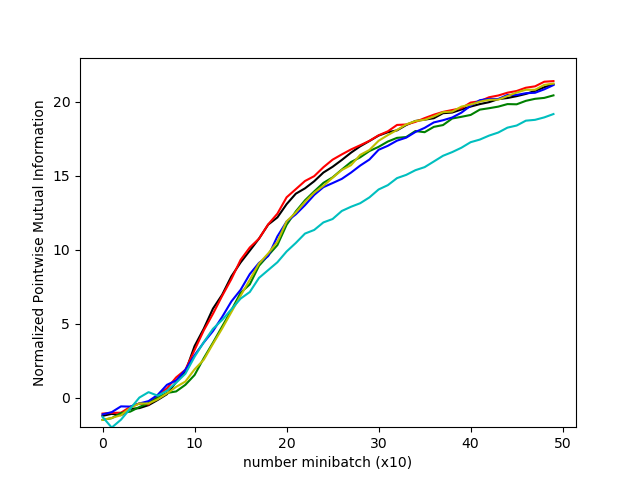
\includegraphics[width=1.1\textwidth]{yahooNPMI100vb.png}}
		\end{figure}				
	\end{column} %
\end{columns}
 \begin{figure}
	\begin{center}
		\captionsetup{justification=centering}
		
\includegraphics[width=100mm]{menu.png}
		\caption{Kết quả độ đo chất lượng chủ đề cho bộ dữ liệu Twitter}
	\end{center}
\end{figure}
\end{frame}

\begin{frame}{Thời gian chạy với bộ dữ liệu Yahoo}
\begin{tabular}{l|c |c | c | c | c | c | c }
	& K & origin & r = 0.1 & r = 0.3 & r = 0.5 & r = 0.7 & r = 0.9 \\
	\hline \hline
	Gibbs &50 & 24259& 22605 & 18919 & 14154 & 9594 & 3856 \\ 
	\hline
	VB &50 & 546& 534 & 501 & 432 &388 & 176 \\
	\hline \hline
	Gibbs &100 &32042 & 27544 & 21763 & 16729 & 19533&  7565\\ 
	\hline
	VB &100 &448 & 418 & 372 & 328 &274 &223\\
	\hline \hline
	Gibbs &150 &73385 & 68762 & 58344 & 44619 & 30748& 12387 \\ 
	\hline
	VB &150 &514 & 490 & 453 & 398 &337 &265\\
	\hline \hline
	Gibbs &200 & 64068& 51862 & 46133 & 6406 & 41653 & 8894 \\ 
	\hline
	VB &200 &580 & 559 & 485 & 434 & 373 &306\\
\end{tabular}
\end{frame}

\begin{frame}{Độ đo khả năng phán đoán mô hình}

\begin{columns}[T] % align columns
	\begin{column}{.50\textwidth}
		\begin{figure}
			\subfloat[Online Gibbs-sampling và R-Gibbs-sampling]{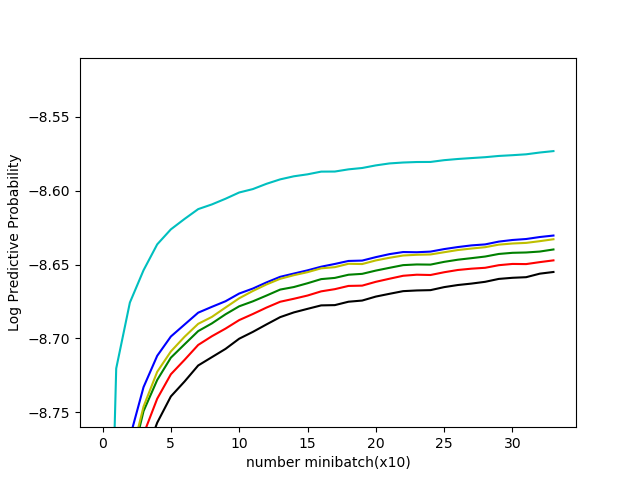
\includegraphics[width=1.1\textwidth]{nytPer100gibb.png}}
		\end{figure}
	\end{column} %
	\hfill%	
	\begin{column}{.50\textwidth}
		\begin{figure}
			\subfloat[Online VB và RVB]{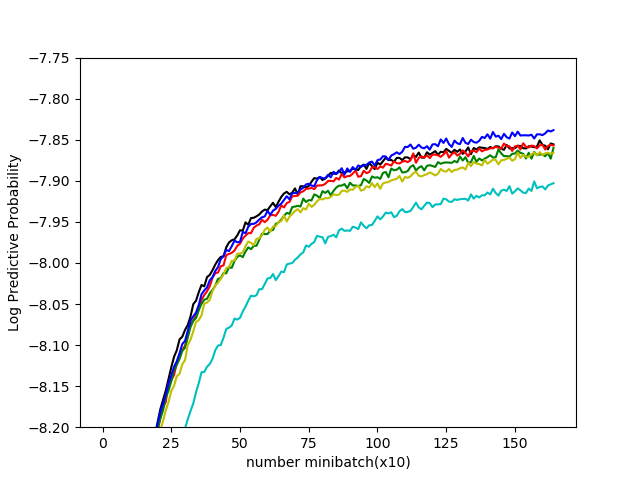
\includegraphics[width=1.1\textwidth]{nytPer100vb.png}}
		\end{figure}				
	\end{column} %
\end{columns}
 \begin{figure}
	\begin{center}
		\captionsetup{justification=centering}
		
\includegraphics[width=100mm]{menu.png}
		\caption{Kết quả độ đo khả năng phán đoán mô hình cho bộ dữ liệu NYT}
	\end{center}
\end{figure}
\end{frame}


\begin{frame}{Độ đo chất lượng chủ đề }
\begin{columns}[T] % align columns
	\begin{column}{.50\textwidth}
		\begin{figure}
			\subfloat[Online Gibbs-sampling và R-Gibbs-sampling]{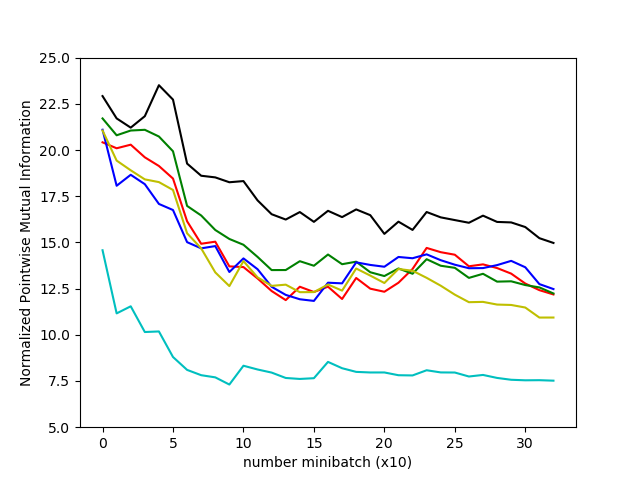
\includegraphics[width=1.1\textwidth]{nytNPMI100gibb.png}}
		\end{figure}
	\end{column} %
	\hfill%	
	\begin{column}{.50\textwidth}
		\begin{figure}
			\subfloat[Online VB và RVB]{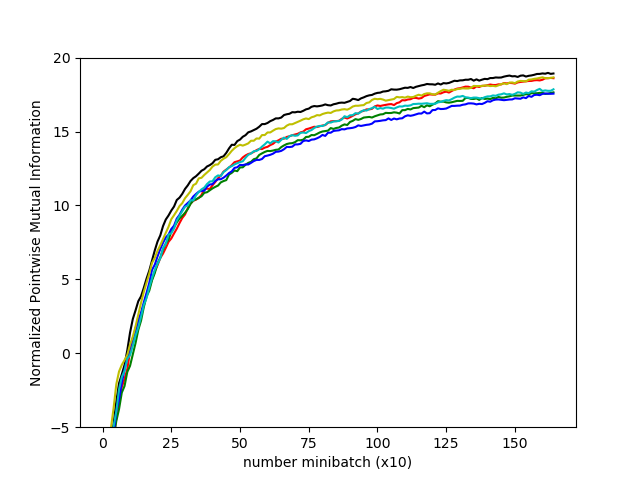
\includegraphics[width=1.1\textwidth]{nytNPMI100vb.png}}
		\end{figure}				
	\end{column} %
\end{columns}
 \begin{figure}
	\begin{center}
		\captionsetup{justification=centering}
		
\includegraphics[width=100mm]{menu.png}
		\caption{Kết quả độ đo chất lượng chủ đề cho bộ dữ liệu NYT}
	\end{center}
\end{figure}
\end{frame}


\begin{frame}{Thời gian chạy với bộ dữ liệu NYT}
\begin{tabular}{l|c |c | c | c | c | c | c }
		& K & origin & r = 0.1 & r = 0.3 & r = 0.5 & r = 0.7 & r = 0.9 \\
		\hline \hline
		Gibbs &50 & 81029& 75909 & 63424 & 49757 & 33146 & 11787 \\ 
		\hline
		VB &50 & 1190&  1876 & 1723 & 1506 &1355 & 633 \\
		\hline \hline
		Gibbs &100 &90219 & 85610 & 71573 & 56306 & 39515&  15900\\ 
		\hline
		VB &100 &1701 & 1569 & 1398 & 1229 &996 &880\\
		\hline \hline
		Gibbs &150 &130083 & 123790 & 124131 & 107083& 89761& 38267 \\ 
		\hline
		VB &150 &1800 & 1792 & 1660 & 1499 &1250 &1030\\
		\hline \hline
		Gibbs &200 & 193110& 180111 & 184658 & 151754 & 47640 & 33396 \\ 
		\hline
		VB &200 &2308 & 2171 & 1707 &  1554 & 1361&1096 \\
\end{tabular}
\end{frame}

\end{document}
